\documentclass[conference]{IEEEtran}
\IEEEoverridecommandlockouts
% The preceding line is only needed to identify funding in the first footnote. If that is unneeded, please comment it out.
\usepackage{cite}
\usepackage{amsmath,amssymb,amsfonts}
\usepackage{array,multirow,graphicx}
\usepackage{float}
%\usepackage{algorithmic}
\usepackage[ruled,vlined]{algorithm2e}
\usepackage{textcomp}
%\usepackage{xcolor}
\usepackage[table]{xcolor}
\usepackage{colortbl}
\def\BibTeX{{\rm B\kern-.05em{\sc i\kern-.025em b}\kern-.08em
    T\kern-.1667em\lower.7ex\hbox{E}\kern-.125emX}}

\definecolor{Gray}{gray}{0.85}
\newcommand{\taskprefix}{CH}
\newcommand{\tasksize}{\normalsize}
\newenvironment{taskenv}[1]{\begin{list}{{\tasksize\sc \theenumi.}}{\usecounter{enumi}
      \settowidth{\labelwidth}{{\tasksize\sc \taskprefix#1-99}}
      \setlength{\leftmargin}{\labelwidth}
      %\addtolength{\leftmargin}{2.0\labelsep}
}}{\end{list}}
\newcounter{task}
\setcounter{task}{-1}
\newcommand{\btask}{\begin{taskenv}{\taskprefix}\setcounter{enumi}{\value{task}}\renewcommand{\theenumi}{\taskprefix$_{\arabic{enumi}}$}}
\newcommand{\etask}{\setcounter{task}{\value{enumi}}\renewcommand{\theenumi}{\arabic{enumi}.}\end{taskenv}}

\begin{document}

\title{Large-scale hybrid ad hoc network for mobile platforms: Challenges and Experiences}

\author{\IEEEauthorblockN{Nirmit Desai, Wendy Chong, Heather Achilles, Shahrokh Daijavad}
\IEEEauthorblockA{\textit{IBM T. J. Watson Research Center} \\
%\textit{}\\
Yorktown Heights, NY, USA \\
\{nirmit.desai, wendych, hachilles, shahrokh\}@us.ibm.com}
\and
%\IEEEauthorblockN{Wendy Chong}
%\IEEEauthorblockA{\textit{IBM T. J. Watson Research Center} \\
%\textit{name of organization (of Aff.)}\\
%Yorktown Heights, NY, USA \\
%wendych@us.ibm.com}
%\and
%\IEEEauthorblockN{Heather Achilles}
%\IEEEauthorblockA{\textit{IBM T. J. Watson Research Center} \\
%\textit{name of organization (of Af}\\
%Yorktown Heights, NY, USA \\
%hachilles@us.ibm.com}
%\and
%\IEEEauthorblockN{Shahrokh Daijavad}
%\IEEEauthorblockA{\textit{IBM T. J. Watson Research Center} \\
%\textit{Penn}\\
%Yorktown Heights, NY, USA \\
%shahrokh@us.ibm.com}
\and
\IEEEauthorblockN{Thomas La Porta}
\IEEEauthorblockA{\textit{Dept. of Computer Science and Engineering} \\
\textit{Penn State University}\\
University Park, PA, USA \\
tlp@cse.psu.edu}
%\and
%\IEEEauthorblockN{5\textsuperscript{th} Given Name Surname}
%\IEEEauthorblockA{\textit{dept. name of organization (of Aff.)} \\
%\textit{name of organization (of Aff.)}\\
%City, Country \\
%email address}
%\and
%\IEEEauthorblockN{6\textsuperscript{th} Given Name Surname}
%\IEEEauthorblockA{\textit{dept. name of organization (of Aff.)} \\
%\textit{name of organization (of Aff.)}\\
%City, Country \\
%email address}
}

\maketitle

\begin{abstract}
Peer-to-peer (p2p) networks and Mobile ad hoc networks (MANET) have
been widely studied. However, a real-world deployment for the masses
has remained elusive. Ever-increasing density of mobile devices,
especially in urban areas, has given rise to new applications of p2p
communication. However, the modern smartphone platforms have limited
support for such communications. Further, the issues of battery life,
range, and trust remain unaddressed. A key question then is, what
kinds of applications can the modern mobile platforms support and what
challenges remain? This paper identifies a class of applications and
presents a novel center-to-peer-to-peer (c2p2p) architecture called
Mesh Network Alerts (MNA) to support them.  We describe our
experiences in deploying MNA as a real-world system to millions of
users for relaying severe weather information along with the
challenges faced, and the approaches for addressing them.
\end{abstract}

\begin{IEEEkeywords}
peer-to-peer systems, mobile ad hoc network, delay-tolerant network
\end{IEEEkeywords}

\section{Introduction}
Mobile devices with programmable platforms such as Android and iOS
have steadily grown over the last decade, surpassing the 2 billion
mark\footnote{https://www.statista.com/statistics/330695/number-of-smartphone-users-worldwide/}. MANETs
have been widely studied given their decentralized nature and
potential for new applications
\cite{loo-manet-2011,perkins-ad-hoc-2001}. Most of the prior work on
p2p networks has focused on analytical and simulation-based study of
MANET behavior
\cite{zhang-topology-manet-2015,marti-misbehavior-manet-2000,mauve-pos-routing-manet-2001}. Given
the outstanding practical challenges in deploying a large number of
physical nodes, real-world implementations have been limited and have
not reached mass scale \cite{kiess-manet-impl-2007}. However, with the
growth of smartphones, large-scale real-world implementations may
become feasible. This paper describes a real-world implementation of a
p2p delay-tolerant network, called Mesh Network Alerts (MNA), for
relaying severe weather information to millions of mobile device users
as part of the Weather Channel app \cite{mna} on both Android and iOS
platforms.

Before describing MNA, it is critical to identify applications that
need p2p communication, given pervasive Internet connectivity and the
ease of using it. Doing so enables us to define key characteristics of
such applications and focus on the challenges in meeting them.  This
paper focuses on two separate classes of applications: communication
in (a) disaster-affected or remote areas and (b) congested networks in
densely populated areas, e.g., sports arenas.  The following are the
key characteristics in these scenarios:

%
\btask
%
\item\label{c:0} No communication infrastructure such as WiFi
  access points to fall back on
\item\label{c:1} Device users are mobile, pattern of mobility is not
  predictable
\item\label{c:2} New information may arrive at any time
\item\label{c:3} Trustworthy information is scarce, misinformation and
  rumours are common place
\item\label{c:4}  Small payloads suffice in many cases and information
  retains value for a few minutes
\item\label{c:5}  Device battery is a scarce resource, power supply
  for recharging may not be available
\item\label{c:6}  Devices are owned by citizens, deployment of
  special-purpose devices is cost prohibitive
%
\etask
%

The above needs are well-recognized in the industry as well as
academia with several ambitious attempts to address them, e.g., Google
Loon project\footnote{https://loon.co} and Facebook
Aquilla\footnote{https://en.wikipedia.org/wiki/Facebook\_Aquila},
though with limited impact. Leveraging user mobile devices as peer
nodes for a large-scale deployment has been another theme in the prior
works, e.g., the Serval project
\cite{gardner-stephen-serval-2011}. Serval mesh enables p2p
communication over on-device WiFi radio, but requires root access to
the device via jail-breaking. Although significant lessons have been
learned through these attempts, a mass-scale p2p network for such
applications remains elusive.

A vast majority of the literature has focused on a traditional model
of stateful, fully decentralized, reliable networking. Specifically,
the nodes maintain connectivity with peers and routing is optimized
with techniques based on link state (OLSR) or distance vectors (AODV)
\cite{clausen-olsr-2003,perkins-aodv-2003} focusing on optimizing the
network utilization.

Given the application characteristics above, this paper identifies
practical challenges associated with modern device platforms and finds
novel ways to overcome them.  This leads to MNA -- a new paradigm in
p2p networking that employs a delay-tolerant, and zero-routing
overhead architecture.  Unlike previous works, MNA is a hybrid of a
centralized and a decentralized architecture, called
\emph{center-to-peer-to-peer (c2p2p)}. A central service is leveraged
as the trusted source of information while the information is
propagated in a decentralized fashion by peers. Such an architecture
allows MNA to bypass the key issue of trust deficit in open
decentralized systems while retaining the ability of
infrastructure-less communication in many application scenarios.

MNA is implemented on both Android and iOS as an SDK and integrated
with the Weather Channel mobile apps. With extensive experiments and
experience of deploying to almost $10$ million users, MNA represents a
way forward for large-scale p2p networks.

This paper makes the following key contributions:
\begin{itemize}
\item Identification of a class of applications for p2p and their key
  characteristics
\item A deeper investigation of the practical challenges in supporting
  the above class of applications
\item A novel c2p2p implementation using multiple radio
  channels on modern mobile platforms (Android and iOS)
\item Experimental evaluation and real-world deployment statistics
\end{itemize}

In the following, Section~\ref{sec:challenges} describes the practical
challenges. Section~\ref{sec:architecture} outlines the architectural
details of MNA along with platform-specific implementation issues for
Android and iOS in addressing the challenges. Section~\ref{sec:algo}
dives into the algorithms of two of the MNA protocols. Experimental
evaluation and deployment statistics are presented in
Section~\ref{sec:eval}.  A deeper look at the literature and contrast
to MNA is summarized in Section~\ref{sec:related} with conclusions in
Section~\ref{sec:conclude}.
%
\section{Challenges}
\label{sec:challenges}
%
We present the main challenges for modern mobile device platforms in
supporting the classes of applications described above. These have been
uncovered via extensive experiments and in some cases include direct
feedback from the developers of Android and iOS.
%
\subsection{Operating system restrictions}
\label{ch:os}
%
Due to \ref{c:2}, even when a user is not interacting with an app, or
worse yet, when the device is not being used at all, the devices must
continue to discover peers to receive and forward
information. Although modern mobile operating systems such as Android
and iOS offer APIs to discover and advertise information to peers over
WiFi and Bluetooth interfaces, peer-to-peer connections do not work
reliably when the same APIs are accessed while the app is in the
background. Further, on Android, each WiFi p2p connection must be
explicitly approved by the user. Prior works widely document
these challenges and take the approach of having special access on the
devices, e.g., jail-breaking or rooting
\cite{gardner-stephen-serval-2011}. Clearly, such an approach does not
scale to mass adoption.\\
%
\subsection{Power constraints}
\label{ch:power}
%
Since devices may be offline when new weather information arrives, MNA
on each peer must remain active at all times to be able to discover
new information as soon as it arrives. Further, as there is no back up
infrastructure (\ref{c:0}) and a set of peers in range can change at
any time (\ref{c:1}), each peer is responsible for constantly
forwarding available information to other peers via
advertisements. However, due to \ref{c:5}, the MNA activity must keep
the device battery consumption to a minimum. This is a challenge
because advertising and discovery are power-hungry operations over the
radio channels.
%
\subsection{Testing p2p networks}
%
Given the heterogeneity of devices owned by users and operating system
distributions (\ref{c:6}), it is challenging to test whether or not
MNA works as expected on a single device. Further, running test
scenarios on a p2p network at large-scale is non-trivial given that a
large number of devices need to take coordinated action
followed by coordinated observations to determine whether a test
passes or fails. Further, since range and mobility affect p2p
communications and they are unpredictable (\ref{c:1}), it is important
to run test cases under various mobility patterns across all nodes in
the network.  Emulated mobility frameworks such as CORE
\cite{arenholz-core-2008} and EMANE \cite{emane} fall short as the
connection latency and wireless transmission are specific to device
hardware.  This is not a challenge in traditional mobile
application development as the application functionality is confined
within a single connected device.
%
\subsection{Trust in information}
%
As user devices advertise on unsecured wireless protocols, it may be
possible for a malicious attacker to listen for such advertisements
and reverse-engineer the protocols used. Then, the attackers may
generate fake messages and advertise them, e.g., a fake tornado
alert. Given a lack of trusted information in such scenarios
(\ref{c:3}), misinformation campaigns can have disastrous
consequences.  In open decentralized systems, such false messages
cannot be distinguished from the real ones, and MNA will end up
propagating them to as many devices as possible, ``poisoning'' the
network. In general, veracity of such information cannot be
independently verified in open decentralized systems and previous
works on peer-to-peer networks do not address this challenge.
%
\section{C2P2P System Architecture}
\label{sec:architecture}
%
\begin{figure}[htbp]
\centerline{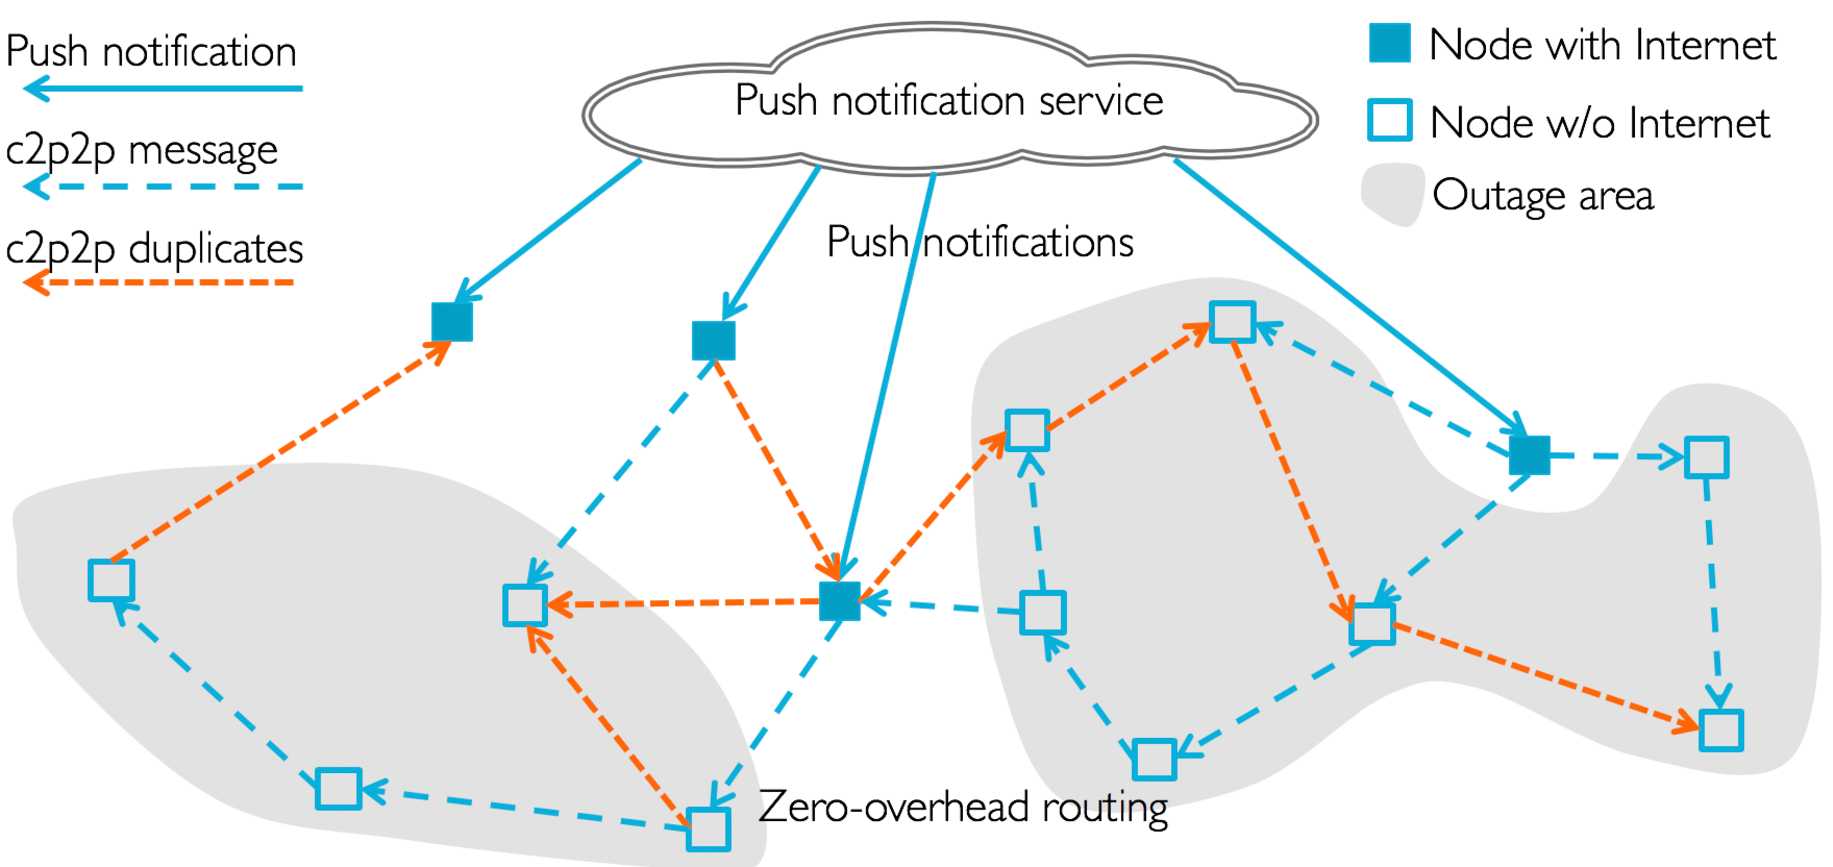
\includegraphics[width=\columnwidth]{figs/arch}}
\caption{c2p2p system architecture}
\label{fig:arch}
\end{figure}

To address (or bypass) the challenges identified above, this paper
proposes c2p2p -- a hybrid architecture that leverages a central
service as the sole source of trusted information as depicted in
Figure~\ref{fig:arch}. An application-specific central service, e.g.,
weather.com backend, originates new information and
assigns it a unique identifier. Next, the central service produces a
digital signature using its private key and appends it to the message
payload. Finally, header parameters specifying TTL (duration after
which the message expires), peer identifier of the central service,
destination peer identifier list (for uni-cast) or a special identifier
(for broadcast), and the time of origin are added to the message and
the message is sent to a push notification service for distribution.

Mobile applications integrate MNA as an SDK with the public key of the
corresponding central service. Peers having Internet connectivity
receive the push messages and verify the digital signature.  If the
signature is valid, the message has not expired, and is destined to
other peers, then the receiving peers forward the message to other
peers. Depending on the protocol being used, such forwarding happens
as a uni-cast or broadcast. Peers receiving the forwarded messages
also verify the digital signature before forwarding further.

Since new information can arrive at any time, new peers may come into
proximity, or message transmissions fail, all peers store unexpired
and verified messages and forward them to proximal peers
repeatedly. This implies that peers may receive a message more than
once but since the messages are globally unique, duplicates can be
identified and ignored.  A peer sending a message adds its own peer
identifier to a list of forwarders appended to the message header.  A
receiving peer thus knows all the peers that already have the message
and stops repeating the message to those peers, controlling the
flooding.  As there are no control messages or any other overhead for
routing, we call this \emph{zero-overhead} routing.

The following assesses the c2p2p architecture relative to the
challenges identified above along with known limitations. Further, to
realize this architecture on mobile devices, we evaluate a variety of
protocols on both Android and iOS. As described later, WiFi DNS on
Android, Bluetooth Nearby on Android, and Bluetooth low energy (BTLE)
on both Android and iOS are the only protocols that were found
effective. Actual techniques for discovery, advertisement, and
connection vary across these protocols and are described next.
%
\subsection{Operating system restrictions}
\label{sec:os}
%
%
\begin{table}[H]
\caption{Android protocols and key findings}
\label{tab:android}
\centering
\begin{tabular}{|c|l|r|r|r|c|l|}
\hline
& \multicolumn{1}{c|}{Protocol} & \multicolumn{1}{c|}{Throughput} & \multicolumn{1}{c|}{Battery} & \multicolumn{1}{c|}{Range} & \multicolumn{1}{c|}{iOS} & \multicolumn{1}{c|}{Issues}\\
&                               & \multicolumn{1}{c|}{Avg. kbps}  & \multicolumn{1}{c|}{per hour} & \multicolumn{1}{c|}{LoS ft} &                  &                            \\
\hline
\parbox[t]{2mm}{\multirow{3}{*}{\rotatebox[origin=c]{90}{WiFi}}} & \textbf{DNS} & 0.2 & 2\% & 600 & No & \\
& WiDi & 2000 & 3\% & 600 & No & Needs DNS\\
& Hotspot & 2000 & 5\% & 600 & No & Permission\\
\hline
\parbox[t]{2mm}{\multirow{3}{*}{\rotatebox[origin=c]{90}{BT}}} & \textbf{Classic} & 50 & 2\% & 600 & No & \\
& \textbf{Nearby} & 50 & 2\% & 600 & No & \\
& \textbf{BTLE} & 50 & 2\% & 600 & Yes & \\
\hline
\end{tabular}
\end{table}
%

MNA works around the background activity and user permission
restrictions via innovative techniques, without resorting to hacks
that may violate user security or developer guidelines.
Tables~\ref{tab:android} and~\ref{tab:ios} summarize the various
protocols we have experimented with using WiFi and Bluetooth
interfaces, along with key findings as described here.  The protocols
actually deployed are in bold.

%
\begin{table}[H]
\caption{iOS protocols and key findings}
\label{tab:ios}
\centering
\begin{tabular}{|c|l|r|r|r|c|l|}
\hline
& \multicolumn{1}{c|}{Protocol} & \multicolumn{1}{c|}{Throughput} & \multicolumn{1}{c|}{Battery} & \multicolumn{1}{c|}{Range} & \multicolumn{1}{c|}{Android} & \multicolumn{1}{c|}{Issues}\\
&                               & \multicolumn{1}{c|}{Avg. kbps}  & \multicolumn{1}{c|}{per hour} & \multicolumn{1}{c|}{LoS ft} &                  &                            \\
\hline
\parbox[t]{2mm}{\multirow{2}{*}{\rotatebox[origin=c]{90}{WiFi}}} & Bonjour & 0.2 & 5\% & 200 & No & Battery\\
& MPC & 2000 & 5\% & 200 & No & Battery\\
\hline
& \textbf{BTLE} & 50 & 1\% & 800 & Yes & \\
\hline
\end{tabular}
\end{table}
%

Throughput is measured over a single p2p hop. Line of Sight (LoS)
range in feet was measured by manually placing devices at increasing
distances until they fail to communicate. Battery consumption per hour
was measured as a difference between baseline battery consumption and
when MNA was left running for 12 hours. Reported numbers are an
average percentage consumption across about 50 devices on each
platform.

BTLE is the only cross-platform protocol, although there are
limitations with operating system versions as shown in
Table~\ref{tab:android_ios}. Android is denoted as A, 18 and 21 API
levels corresponding to Android versions 4.3 and 5.0 respectively, and
C and P denote the roles of Central and Peripheral. Key finding is
that Android 4.3 devices acting as Peripheral cannot communicate
either as senders or receivers.
%
\begin{table}[H]
\caption{BTLE interoperability between Android and iOS devices}
\label{tab:android_ios}
\centering
\begin{tabular}{|c|c|c|c|c|c|c|}
\hline 
\multicolumn{1}{|c|}{Sender} & \multicolumn{6}{c|}{Receiver} \\
\hline
\multicolumn{1}{|c|}{} & A.18-C & A.18-P & A.21-C & A.21-P  & iOS-C & iOS-P \\
\hline
A.18-C & \cellcolor{Gray}         &   No       & \cellcolor{Gray}         &    Yes       &  \cellcolor{Gray}       &   Yes      \\ 
\hline
A.18-P &  No        & \cellcolor{Gray}         &   No       &  \cellcolor{Gray}         &   No      &  \cellcolor{Gray}       \\ 
\hline
A.21-C & \cellcolor{Gray}         &   No       &  \cellcolor{Gray}        &    Yes       &  \cellcolor{Gray}       &   Yes      \\ 
\hline
A.21-P &  Yes        & \cellcolor{Gray}         &   Yes       &  \cellcolor{Gray}         &   Yes      & \cellcolor{Gray}        \\ 
\hline
iOS-C & \cellcolor{Gray}         &    No      &  \cellcolor{Gray}        &     Yes       & \cellcolor{Gray}        &   Yes      \\ 
\hline
iOS-P &   Yes       & \cellcolor{Gray}         &    Yes      &  \cellcolor{Gray}         &   Yes      &  \cellcolor{Gray}       \\ 
\hline
\end{tabular}
\end{table}
%

WiFi Direct (WiDi) is a clever combination of Hotspot with WiFi DNS
wherein peers randomly choose to be a Hotspot or a client, discover
WiFi credentials over WiFi DNS discovery and make WiFi connection to
Hotspot without needing user permission.  However, both Hotspot and
WiDi suffer from higher battery consumption than DNS and hence were
not deployed. All Android protocols leverage foreground services to
continue discovery and advertisement operations in the background
indefinitely. Algorithms for WiFi DNS and BTLE are described in detail
in Section~\ref{sec:algo}.

%
\subsection{Power constraints}
\label{sec:power}
%
Due to indefinite foreground services and continuous discovery and
advertisement, this is primarily an issue on Android. Our approach
here is two-pronged. Firstly, via extensive experiments on a large
number of devices, we fine-tune the algorithms governing the intervals
at which discovery and advertisements occur. In a nutshell, receiving
new information during a period causes MNA to be more aggressive in
discovery and advertisement. Similarly, lack of new information for a
period makes the device less aggressive. Secondly, we allow the
central service to broadcast``wake up'' messages ahead of an
anticipated severe weather event.  When devices receive such messages,
they schedule themselves to remain aggressive during the specified
window of time.  Outside of this window, the devices can afford to have
long sleep cycles and conserve power. With these techniques, our
testing shows less than 2\% battery consumption per hour on most
device models.
%
\subsection{Testing p2p networks}
\label{sec:texting}
%
We developed novel test automation tools and processes that control
multiple devices from a single test station and follow prescribed
steps to generate, send, and receives messages to play out a test
scenario.  The framework allows automated analysis of the observations
to determine the test result. This capability was instrumental in
uncovering bugs at a fast pace with tens of physical devices employed
for automated testing.  Further, the automation framework is general
and can be expressly applied to test other apps in this fashion.

Figure~\ref{fig:test_arch} shows the test automation architecture. A
tester specifies high-level test cases and expected results in a
platform and device-agnostic fashion. Mobile devices run a UI proxy
app for executing platform and device-specific UI commands while a
central laptop terminal acts as the overall orchestrator. The
orchestrator translates high-level test cases and distributes them to
devices. Since the orchestrator needs wired access to the devices and
the devices cannot be programmed to move, testing of range and
mobility patterns needs to done manually, which is a known limitation.

A key innovation here is the platform-independent language for
specifying high-level test cases and a small set of primitive commands
it translates to. We describe here the list of primitive commands and
have made available a screen recording across seven Android devices
demonstrates this powerful capability \cite{mna-test-demo}.
\begin{itemize}
\item \textsf{syncAll} -- Wait for all devices to reach this point
\item \textsf{object.find} -- Find a UI object by name or position
\item \textsf{object.click} -- Click a UI object
\item \textsf{sleep} -- Wait for the specified duration
\item \textsf{setupSystemAlert} -- Respond to a system popup
\item \textsf{text.set} -- Highlight a text input box
\item \textsf{text.write} -- Write text to the text box
\item \textsf{swipe} -- Swipe to the left/right or up/down
\end{itemize}

\begin{figure}[htbp]
\centerline{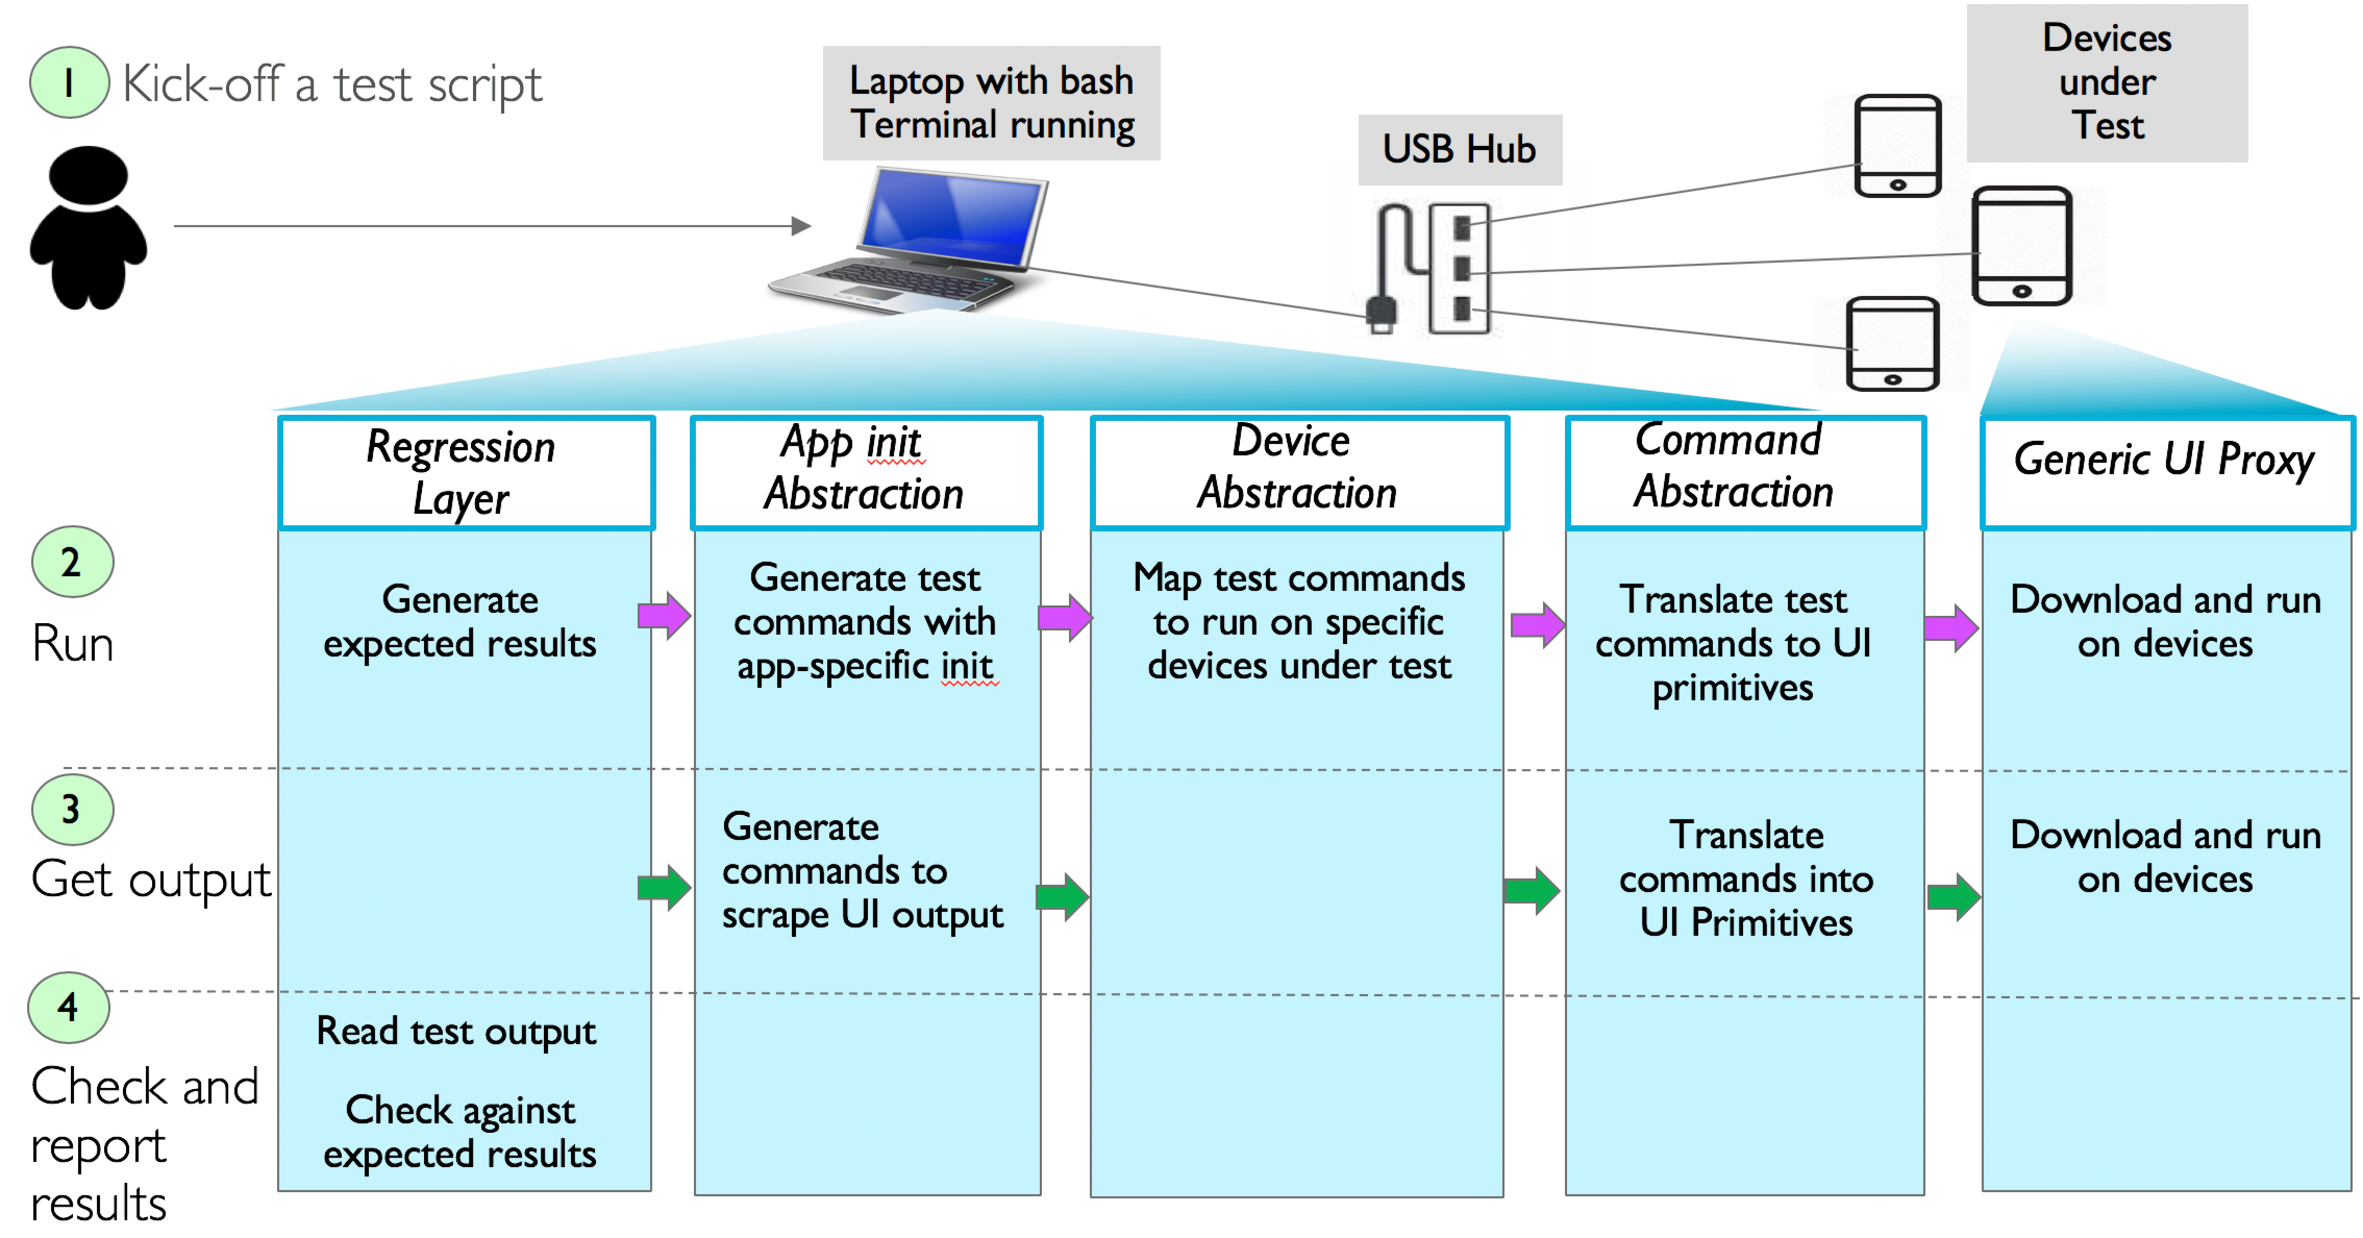
\includegraphics[width=\columnwidth]{figs/test_arch}}
\caption{Automated testing system for MNA}
\label{fig:test_arch}
\end{figure}

%
\subsection{Trust in information}
\label{sec:trust}
%
In c2p2p, since the central service originates all messages, it can
digitally sign them. The mobile application is distributed
with the corresponding public key so that digital signatures from the
service can be verified.  If a message fails such a verification, it
is discarded and not forwarded any further.

Peers cannot originate messages however as then a malicious peer can
join the network, exchange keys with other peers, start generating,
signing, and spreading fake information. This has been a longstanding
problem for open decentralized systems. Requiring all peers to
register their identity with a certificate authority and reporting the
originators of fake information may discourage malicious behavior.
Clearly, this is even harder to solve than the spread of fake
information over the Internet because ground truth is hard to find and
malicious peers can report genuine sources of information as fake.
%
\section{Algorithms}
\label{sec:algo}
%
\subsection{WiFi DNS}
\label{sec:wifi}
%
DNS service discovery is a widely supported protocol
\cite{cheshire-dns-sd-2013}. On Android, WiFi DNS improvises on this
standard such that communication happens without making network
connections. This is achieved by splitting the message payloads into
small enough chunks, stuffing them into service advertisements as txt
records, and broadcasting them over multiple advertisements. Since
there are no connections being made, the messages can be exchanged
without prompting the user to grant permissions for each
connection. Since no peer connections are needed and advertisements
and discovery are broadcast, WiFi DNS is a broadcast
protocol. Although the standard states that as much as 65KB of txt
records can be added to advertisements, in practice most devices
support only up to 750 bytes. On iOS, Bonjour protocol is built on DNS
service discovery but is power-hungry and does not inter-operate with
WiFi DNS on Android. Algorithm~\ref{algo:dns} outlines the peer
process for WiFi DNS. Power conservation via time intervals is
achieved by manipulating timers $T_{ad}$ and $T_{disc}$ based on
traffic. $\mathbb{M}$ is the set of all unexpired messages.

Messages from multiple applications are forwarded on the same network,
but a peer can validate signatures only for the messages targeting an
app it hosts. This is because peers do not possess the public keys
corresponding to the central services of other apps. Hence, peers
simply forward messages not targeting one of their apps. Key benefit
of this design is that the entire network of peers is available to all
apps, making c2p2p scenarios viable even when an individual app does
not have a sufficient density of users.  However, this also allows a
malicious jammer to generate traffic for a fake app, forcing the peers
to forward it until the messages expire.  Although the fake
information will never be delivered to the apps, this affects
throughput. A possible solution would be to distribute a registry of
valid $a_{id}$ to all peers across apps so that they can ignore
messages with fake $a_{id}$ and not forward them.

\begin{algorithm}[htb!]
\label{algo:dns}
\DontPrintSemicolon % Some LaTeX compilers require you to use \dontprintsemicolon instead
\SetAlgoLined
\KwIn{Peer id $p_{id}$, App id $a_{id}$}
\KwIn{max advert/discovery intervals $max_{ad}$, $max_{disc}$}
\KwIn{min advert/discovery intervals $min_{ad}$, $min_{disc}$}
 $S_{name} \gets$ \textsf{'MNA'}\;
 $\mathbb{M} \gets \varnothing$\;
 $T_{ad} \gets min_{ad}$\;
 $T_{disc} \gets min_{disc}$\;
 $New \gets 0$\;
 \ForEach{timer expiry $T_{ad}$}{
   $\mathbb{M} \gets \mathbb{M} -$ expired messages\;
   $\mathbb{M}_{sort} \gets$ $\mathbb{M}$ sorted by least advertised first\;
   $B \gets$ $\mathbb{M}_{sort}$ chunked by MTU size\;
   dnsAdvertise ($S_{name}$, $p_{id}$, $B$)\;
   \If{$New = 0$}{
     $T_{ad} \gets min(T_{ad} \times 2, max_{ad})$\;
   }
 }
 \ForEach{timer expiry $T_{disc}$}{
   dnsDiscover ($S_{name}$, $p_{id}$)\;
   \If{$New = 0$}{
     $T_{disc} \gets min(T_{disc} \times 2, max_{disc})$\;
   }
   $New \gets 0$\;
 }
 \ForEach{discovered service callback $S_{disc}$}{
   $B \gets S_{disc}.B$\;
   $M_{part} \gets msg(B)$\;
   $M \gets M + M_{part}$\; 
   \If{$M_{part}$ is not a duplicate}{
        $T_{ad} \gets max(\frac{T_{ad}}{2}, min_{ad})$\;
        $T_{disc} \gets max(\frac{T_{disc}}{2}, min_{disc})$\;
        $New \gets 1$\;
   }
   \If{$M_{part}$ was the last chunk of $M$}{
     \If{$M$ is unexpired}{
         \If{$M.app = a_{id}$ $\wedge$ $M$ signature is valid}{
             Notify app with $M$\;
         }
         $\mathbb{M} \gets \mathbb{M} \cup M$\;
     }
   }
 }
 \tcc{For testing only}
 \ForEach{app request to send $M$}{
   \If{$M$ has not expired}{
     $\mathbb{M} \gets \mathbb{M} \cup M$\;
   }
 }
 \caption{WiFi DNS peer algorithm}
\end{algorithm}
%
\subsection{BTLE}
\label{sec:btle}
%

The only protocol that stays reliably active in background without
violating developer guidelines is BTLE. Unlike Android, iOS
applications do not need to discover and advertise continually. Once a
BTLE Peripheral (role that has information) is advertised and a
Central (role that receives information) requests discovery, the app
is allowed to go to sleep. When a matching Central or a Peripheral is
found, iOS wakes up the application to handle such an event, even when
the application is in the background. MNA builds on this and leverages
asynchronous dispatch queues to turn each peer into a Central as well
as a Peripheral simultaneously. This architecture allows bidirectional
data transfers without concurrency issues.

Algorithm~\ref{algo:btle} outlines the peer process for BTLE. The
biggest difference with WiFi DNS is that discovery and advertisements
happen only once per app launch. Secondly, the entire peer process is
event-driven, so the app can sleep when there are no events to
process. The list of forwarders for each message $M.fwdList$ is key in
controlling duplicate transmissions without overhead messages. In
practice, limiting number of Peripherals a Central connects to enables
reliable communications, specified by $max_p$.

\begin{algorithm}[htb!]
\label{algo:btle}
\DontPrintSemicolon % Some LaTeX compilers require you to use \dontprintsemicolon instead
\SetAlgoLined
\KwIn{Peer id $p_{id}$, App id $a_{id}$, Max peripherals $max_p$}
 $S_{name} \gets$ \textsf{'MNA'}\;
 $\mathbb{M} \gets \varnothing$\;
 $C \gets$ new Central() in new dispatch queue\;
 $P \gets$ new Peripheral() in new dispatch queue\;
 $T \gets$ new data sender dispatch queue\;
 $C$.bleDiscovery($p_{id}$, $S_{name}$)\;
 $P$.bleAdvert($p_{id}$, $S_{name}$)\;
 $P_{con} \gets 0$\;

 \ForEach{Peripheral $peer$ found event}{
   \If{$P_{con} < max_p$}{
     $C$.connect($peer$)\;
     $P_{con} \gets P_{con} + 1$\;
   }
 }

 \ForEach{Peripheral $peer$ connected event}{
   \ForEach{$M$ $\in$ $\mathbb{M}$}{
     \If{$peer \notin M$.fwdList}{
       $T$.send($M$, $peer$)\;
     }
   }
 }

 \ForEach{Peripheral $peer$ disconnected event}{
    $P_{con} \gets P_{con} - 1$\;
 }

 \ForEach{Central $peer$ connected event}{
   \ForEach{$M$ $\in$ $\mathbb{M}$}{
     \If{$peer \notin M$.fwdList}{
       $T$.send($M$, $peer$)\;
     }
   }
 }

 \ForEach{$M$ received event from $T$.receive()}{
   \If{$M$ is not a duplicate $\wedge$ $M$ is unexpired}{
     \If{$M.app = a_{id}$ $\wedge$ $M$ signature is valid}{
       Notify app with $M$\;
     }
     $M$.fwdList $\gets$ $M$.fwdList $\cup$ $p_{id}$\;
     $\mathbb{M} \gets \mathbb{M} \cup M$\;     
     $T$.send($M$, all connected peers)\;
   }
 }
 \tcc{For testing only}
 \ForEach{app request to send $M$}{
   \If{$M$ has not expired}{
     $M$.fwdList $\gets$ $p_{id}$ \;
     $\mathbb{M} \gets \mathbb{M} \cup M$\;
     $T$.send($M$, all connected peers)\;
   }
 }
 \caption{BTLE peer algorithm}
\end{algorithm}

%
\section{Experimental Results}
\label{sec:eval}
%
Although MNA is deployed to about $10$ million users, collecting test
data runs into privacy and scale issues. Also, given that testing with
a large number of physical devices along with mobility is challenging,
we employ a three-pronged approach to evaluation: (1) gather limited
metrics from the MNA user population, (2) recruit human volunteers in
a pilot to have the tests run on their personal devices, and (3) use
the automated test environment to run controlled experiments. All
experiments mentioning WiFi are on the WiFi DNS channel and BT is
Bluetooth classic.
%
\subsection{MNA limited experiment}
\label{sec:mna}
%
\begin{figure}[htbp]
\centerline{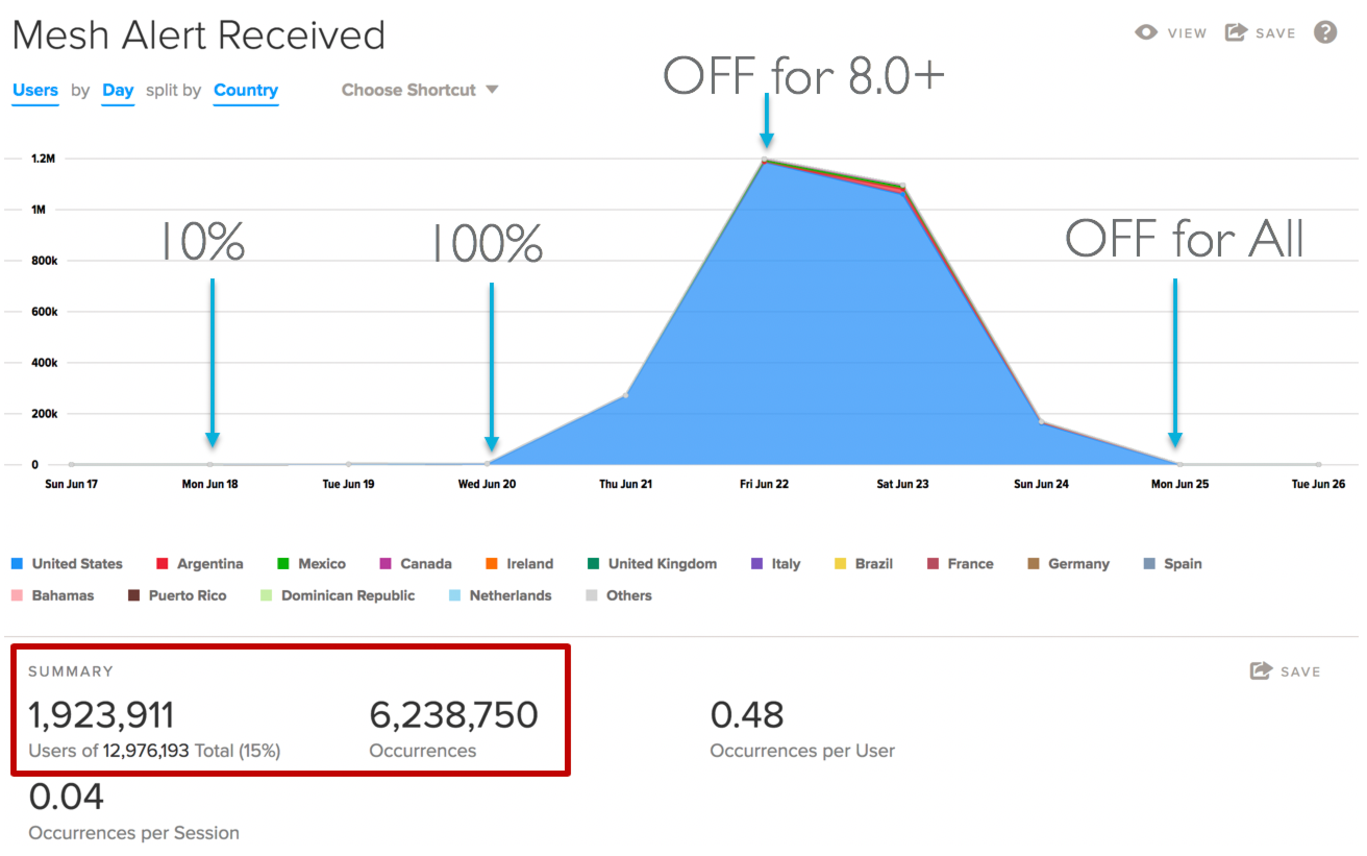
\includegraphics[width=\columnwidth]{figs/mna}}
\caption{Messages received over mesh in one week}
\label{fig:mna}
\end{figure}
%
As Figure~\ref{fig:mna} shows, test data comprising number of messages
received first via MNA and the number of unique users was collected
during a week in June 2018. Almost no MNA messages were received with
a roll-out to $10\%$ of the users.  This makes sense given that p2p
needs critical density of users to propagate messages over large
distances.  With $100\%$ of the users participating, 6 million+
weather alerts were received first via MNA by 1.9 million+ users. Even
when the users are connected to the Internet, they may receive the
alert via MNA before the push notification arrives via the
Internet. Given that such a large population of users received it via
MNA first implies that there is value in the c2p2p architecture even
when Internet connectivity is available.
%
\subsection{Pilot test results}
\label{sec:romania}
%
About 25 colleagues participated in a pilot on a site across two
office buildings and about a thousand people in total.  Clearly, the
user density in this case was low. The app installed on their personal
devices broadcast messages of varying sizes every five minutes
and statistics on MNA were collected. 

Overall, about 13\% of the messages were received at least once while
users actively used the devices for ~5\% of the time.
Figure~\ref{fig:romania_lat} shows how number of messages received and
the single-hop latency vary between WiFi DNS and BT Classic with
increasing packet sizes. Except for the 1000 byte+ packets, WiFi DNS
achieved lower end-to-end latencies than BT Classic, perhaps due to
its broadcast model. This also explains why more messages were
delivered over WiFi DNS than BT Classic. Packet sizes did not affect
single-hop latencies on WiFi DNS, perhaps because most of the messages
fit within a single advertised chunk.

\begin{figure}[htbp]
\centerline{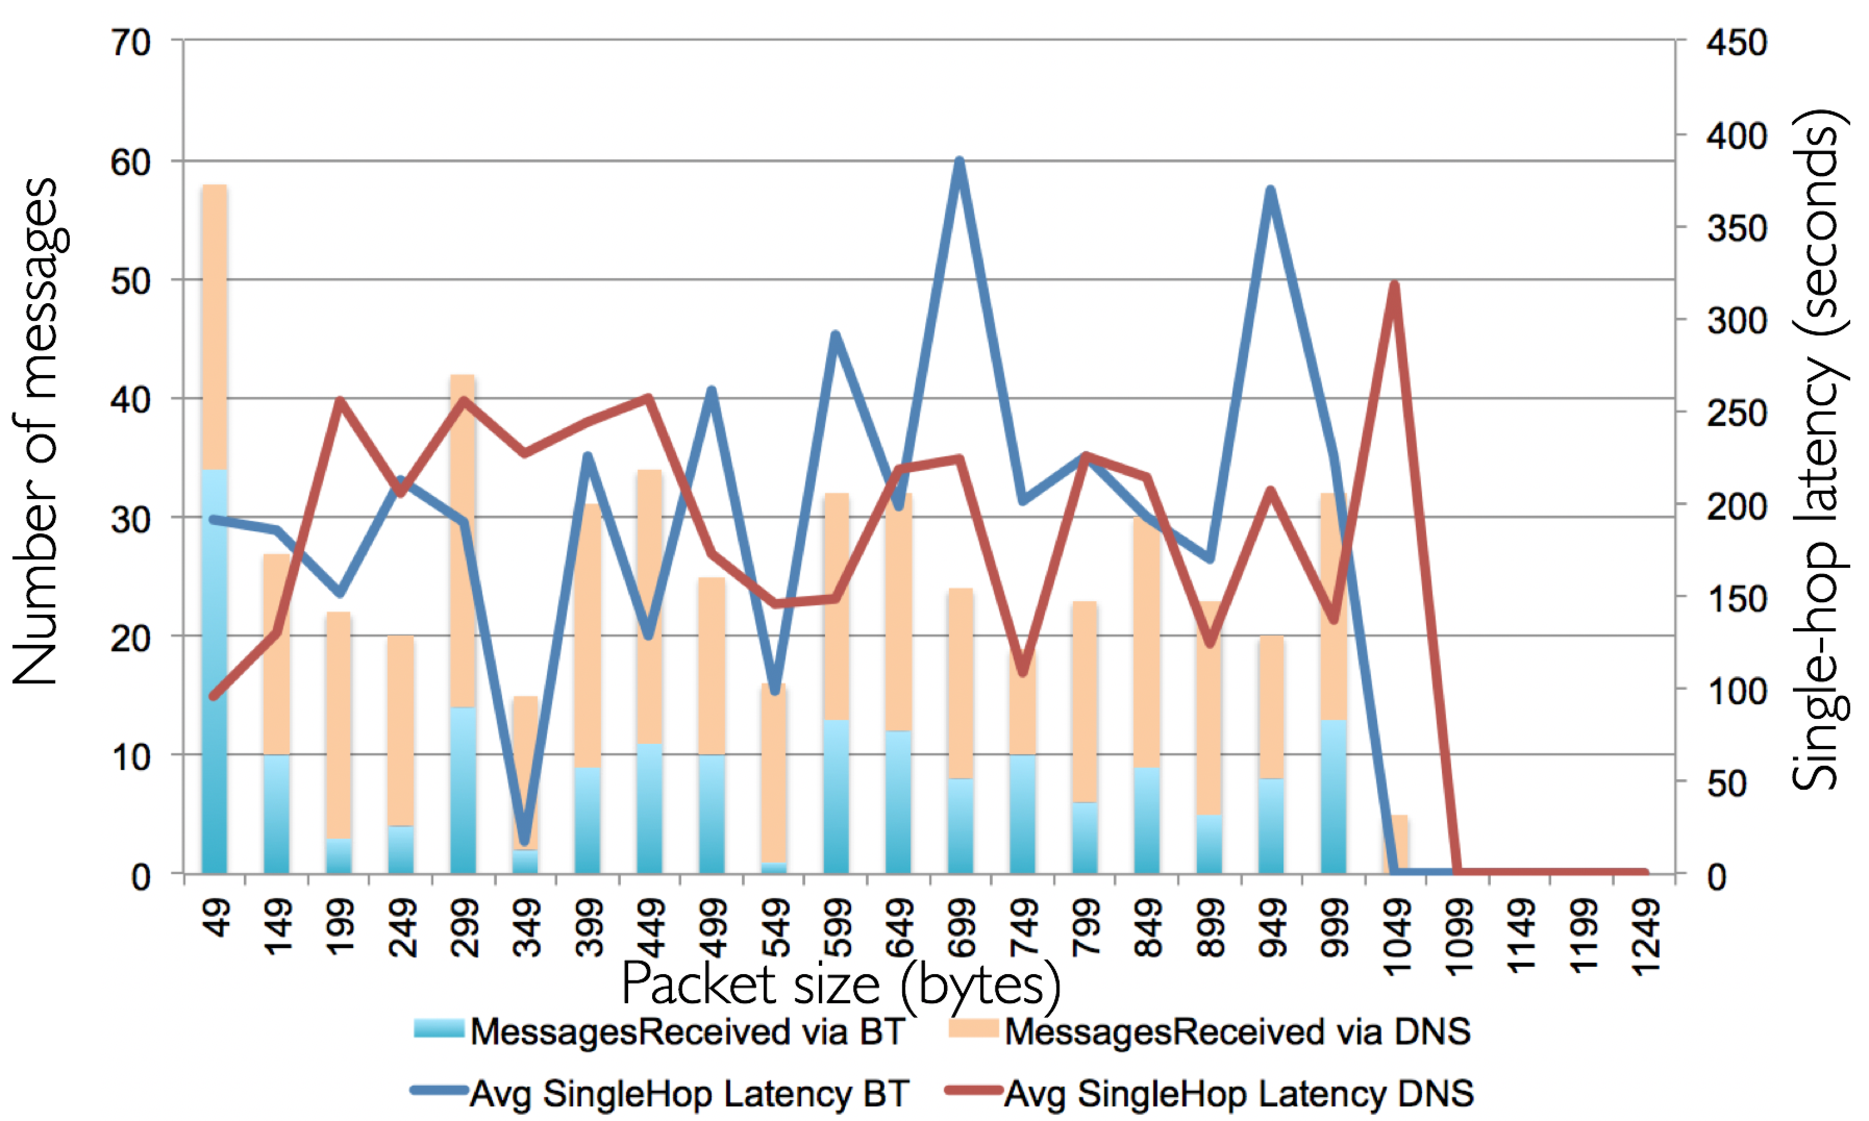
\includegraphics[width=\columnwidth]{figs/romania_latency}}
\caption{Latency as a function of packet sizes}
\label{fig:romania_lat}
\end{figure}

%\begin{figure}[htbp]
%\centerline{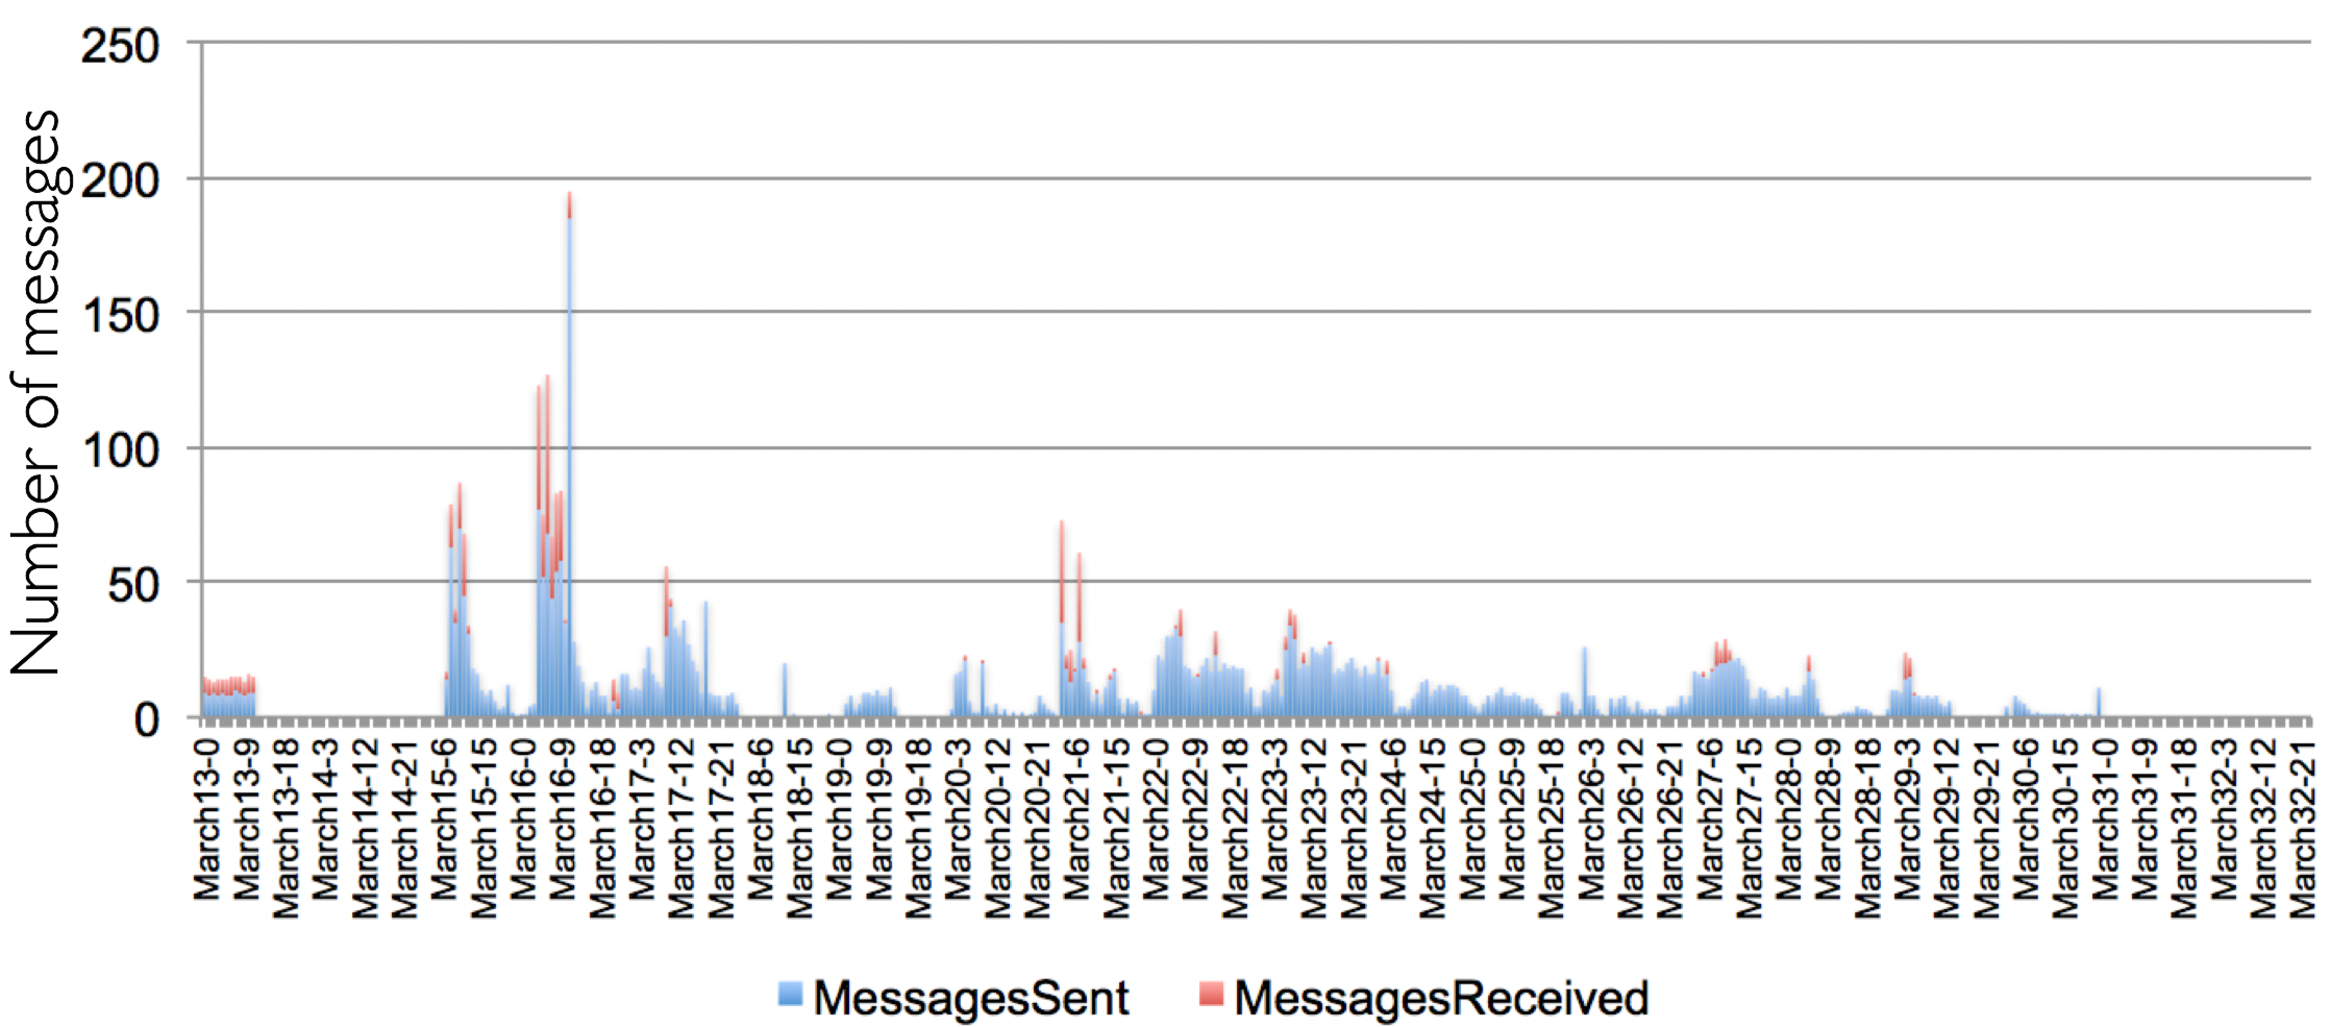
\includegraphics[width=\columnwidth]{figs/romania_activity}}
%\caption{MNA activity during the pilot}
%\label{fig:romania_act}
%\end{figure}

%
\subsection{Automated test results}
\label{sec:automated}
%
We turn to the automated testing with up to 10 physical devices to
carry out some controlled experiments and a deeper understanding of
how the various MNA protocols behave. In these experiments, all
messages has a TTL of 15 minutes and all messages were received within
that duration except for the 10KB messages on WiFi DNS.
%
\begin{figure}[htbp]
\centerline{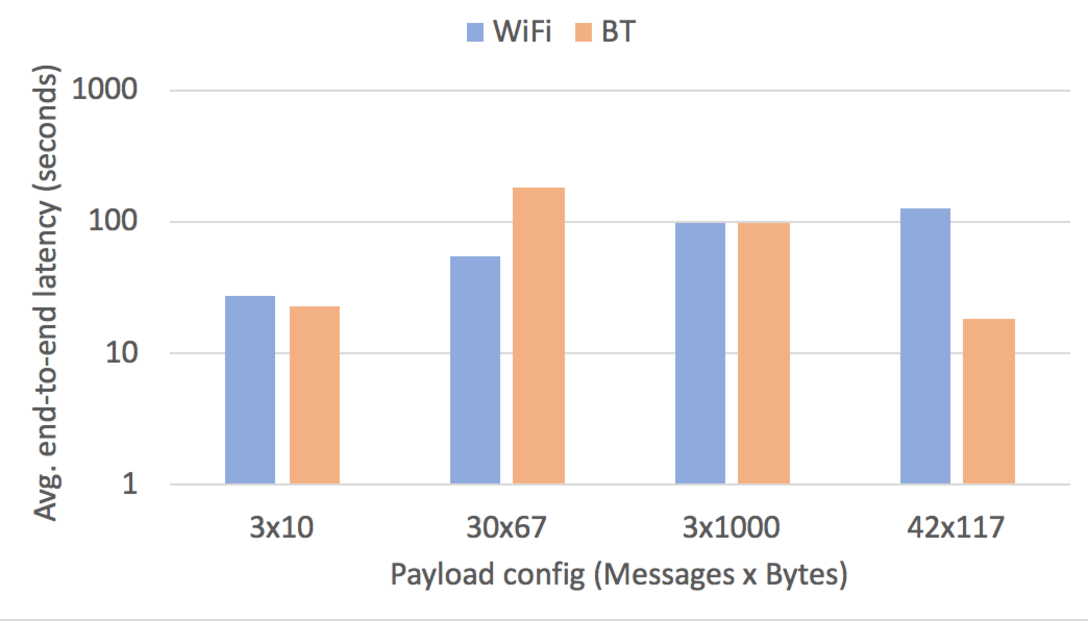
\includegraphics[width=0.8\columnwidth]{figs/variety_e2e_latency}}
\caption{End-to-end latency, WiFi DNS vs. BT Classic}
\label{fig:variety_e2e}
\end{figure}
%

Figure~\ref{fig:variety_e2e} shows end-to-end latency results with
three Android devices, each sending a varying number of messages with
varying sizes. Latency is shown on y-axis on a logarithmic
scale. Total load on network increases from left to right on x-axis
while the number of messages is small for the first and third
cases it is large for the second and fourth cases.

As expected, WiFi DNS latency increases significantly with network
load given its very low throughput. As BT Classic cannot broadcast, it
spends significant time making connections with peers.  Hence, WiFi
DNS beats BT Classic in the 30x67 configuration involving a large
number of small messages. However, when the message sizes are
increased as in 42x117 configuration, BT Classic is almost 10x faster
than WiFi DNS due to superior
throughput. Figure~\ref{fig:variety_hops} confirms this difference in
network topology by measuring average hop counts. WiFi DNS always
needs fewer hops to deliver messages than BT Classic.
%
\begin{figure}[htbp]
\centerline{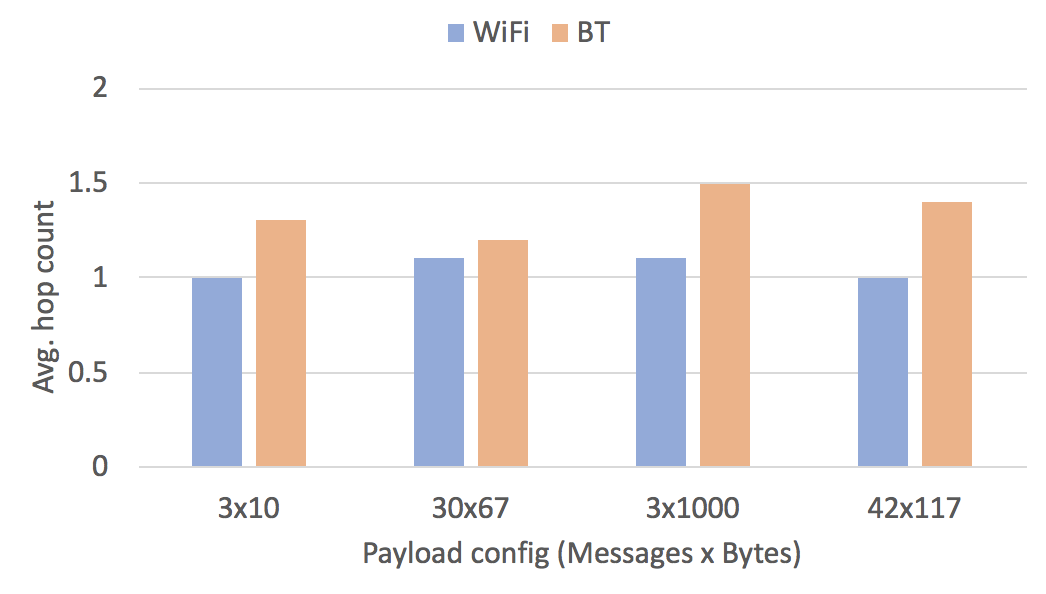
\includegraphics[width=0.8\columnwidth]{figs/variety_hops}}
\caption{Hop counts, WiFi DNS vs. BT Classic}
\label{fig:variety_hops}
\end{figure}
%

Next, we compare WiFi DNS and BT Nearby on Android with BTLE on iOS in
terms of end-to-end latency as the payload size increases as shown
in Figure~\ref{fig:e2e}. The results were collected over three repeats
of the experiment involving up to 10 android devices and 6 iOS
devices. BTLE is almost 100x faster than WiFi DNS and BT Nearby. For
WiFi DNS, as payload size approaches the max advertisement chunk limit
of 750 bytes, the end-to-end latency rises by almost 10x (100 bytes
versus 720 bytes). Behavior of BT Nearby taking time to form
connections but having a good throughput is evident as the end-to-end
latency does not change even when payload sizes go up to 10KB. BTLE on
the other hand gets 10x slower with 10KB payloads as compared to 1KB.

\begin{figure}[htbp]
\centerline{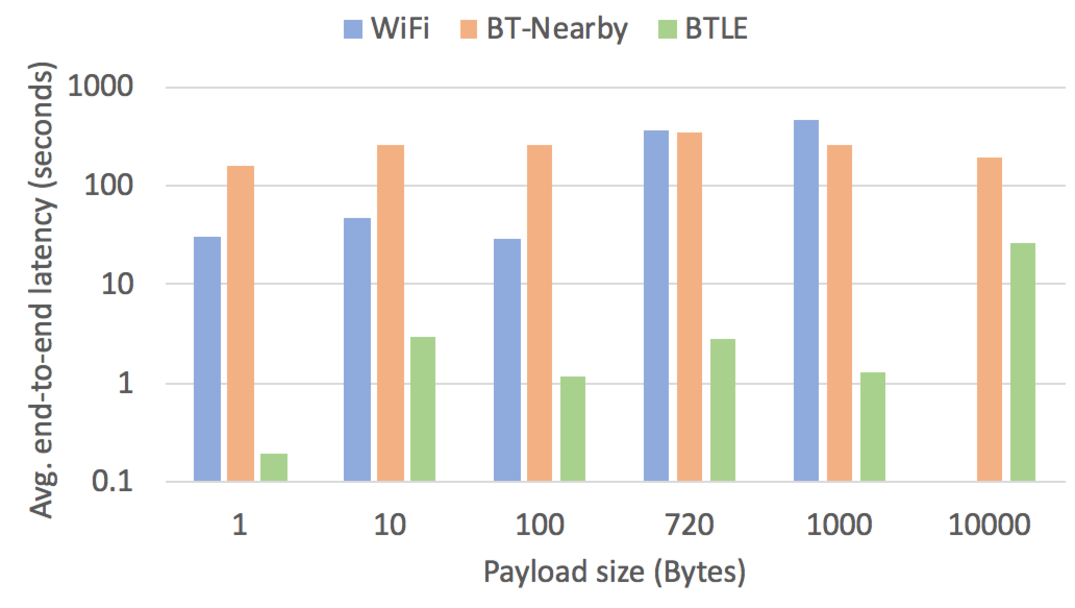
\includegraphics[width=0.8\columnwidth]{figs/e2e_latency}}
\caption{End-to-end latency, WiFi DNS vs. BT Nearby vs. BTLE}
\label{fig:e2e}
\end{figure}

As described above, MNA employs zero-overhead routing with the goal of
maximizing coverage and minimizing latency across peers while
tolerating topology changes.  As a result, messages may be delivered
multiple times to the same peer as no control messages are sent to
keep track of the peer state.  Figure~\ref{fig:dup} shows the cost of
such an approach in terms of average number of duplicate messages
received by peers across WiFi DNS, BT Nearby, and BTLE (iOS). 

For small payload sizes, WiFi DNS ends up duplicating a large number
of messages as the broadcasts are seen by many peers and repeated
advertisements must go on to reach newly proximal peers. The
duplicates drop significantly with payloads approaching the
advertisement chunk size because the fraction of transmissions that
are successfull also drops with large payloads (multiple chunks need
to be delivered per message). The forward list in BT Nearby and BTLE
help control the duplicates significantly.

\begin{figure}[htbp]
\centerline{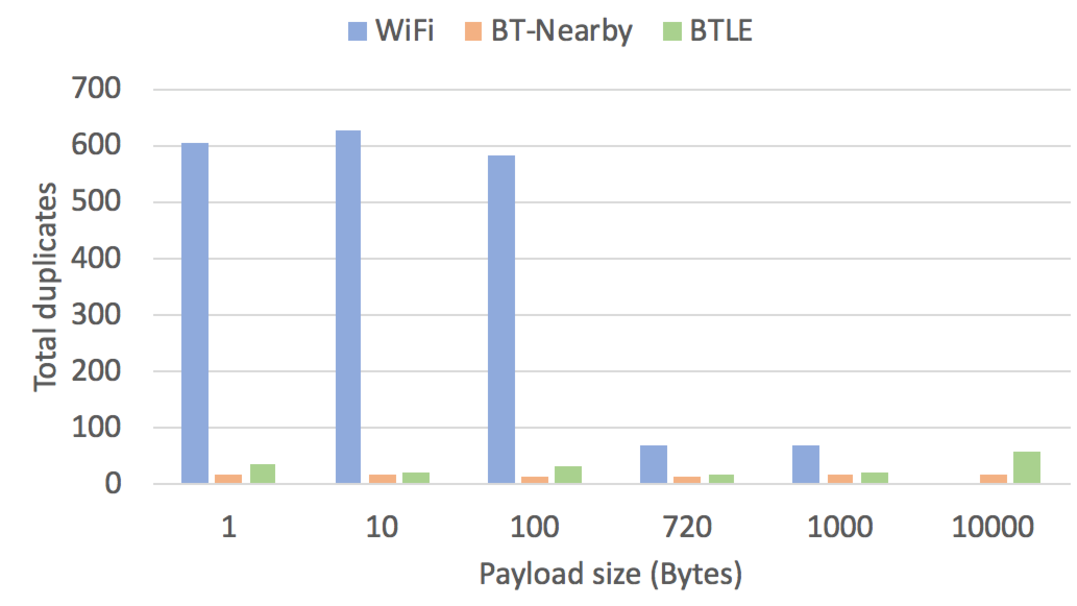
\includegraphics[width=0.8\columnwidth]{figs/duplicates}}
\caption{Duplicity due to zero-overhead routing}
\label{fig:dup}
\end{figure}

Lastly, Figure~\ref{fig:hop} shows the network toplogy underlying WiFi
DNS, BT Nearby, and BTLE. As shown earlier in
Figure~\ref{fig:variety_hops}, WiFi DNS delivers most of the message
with a single hop due to a broadcast protocol whereas BT Nearby and
BTLE need as many as two hops on average.
%
\begin{figure}[htbp]
\centerline{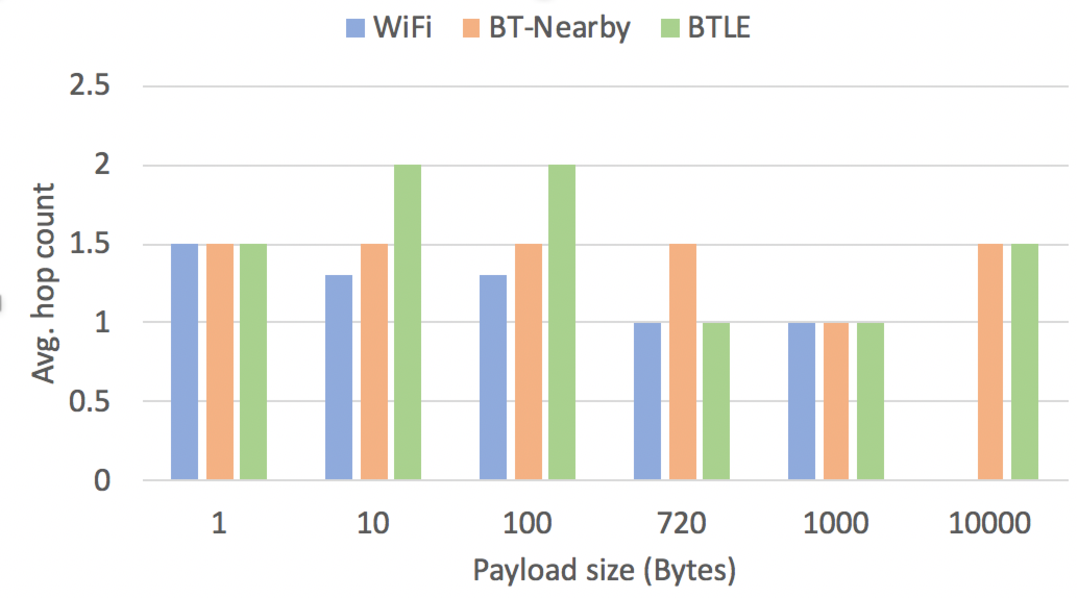
\includegraphics[width=0.8\columnwidth]{figs/hops}}
\caption{Avg hop count, WiFi DNS vs. BT Nearby vs. BTLE}
\label{fig:hop}
\end{figure}
%
%
\section{Related Work}
\label{sec:related}
%
Apart from the state-of-the-art cited earlier, there have been other
notable attempts at practical large-scale deployments, some of which
will be described here. Before mid-2000s, most of the research on
MANETs was based on Department of Defense requirements, until
commodity multi-hop ad hoc networks began to be considered
\cite{bruno-mesh-2005}. Around that time, academia and industry
started publishing and implementing commodity mesh networks in
university and industrial environments. Some notable projects from
this era are: the community-based multi-hop wireless network by Bahl
et al. at Microsoft Research \cite{microsoft-mesh}, the Broadband and
Wireless Network (BWN) project at Georgia Tech \cite{gatech-mesh}, the
testbed created at UCLA Network Research Lab for Wireless Mesh
Networks and the evaluation of its performance of real-time traffic
\cite{chavoutier-2007}, the wireless mesh network testbed at Shanghai
Jiao Tong University \cite{wu-mesh-2010}, and a survey paper about
Wireless Mesh Networks and its challenges at the transport layer
\cite{saha-mesh-2014}.

Despite these efforts, it took until 2014 before wireless mesh
networking was used commercially to enable smartphones to connect via
Bluetooth and WiFi in a popular application called FireChat
\cite{firechat}. The success of FireChat, partially due to the news
coverage of its use in political situations in which governments
restricted access to the Internet, has led to many alternatives in the
past few years. An up-to-date list of such applications is available
here\footnote{https://alternativeto.net/software/firechat-by-open-garden/}.
All of these works are fully decentralized and cannot guarantee
veracity of information being propagated.

Unlike the above-cited works, MNA employs a hybrid architecture
focused on trusted information and low throughput low-power
protocols. With the recent introduction of p2p support at the
operating system level by Apple and Google for smartphones, we believe
there will be a significant increase in both academic and industrial
implementations of large scale mesh networks in the upcoming years.
%
\section{Conclusions and Future Work}
\label{sec:conclude}
%
We reported on MNA, a large-scale real-world hybrid ad hoc network for
Android and iOS platforms. Leveraging a central service as the source
of trusted information with a novel c2p2p architecture enables a class
of applications over an increasing density of mobile devices. MNA
addresses or bypasses operating system restrictions with simple and
creative algorithms without violating user privacy, security, or
developer guidelines. Extensive experiments with real users, pilot
users, and automation show that MNA enables low-throughput
connectivity on modern devices with low battery consumption on both
Android and iOS platforms.

Although MNA represents a significant step forward in the right
direction, there are significant limitations to be overcome. First,
many applications require peers to originate information, e.g., asking
for help during a natural disaster. Hence, the issue of trust in open
decentralized systems needs to be investigated.  Second, although MNA
delivers almost all messages sent to all peers, it cannot guarantee a
100\% delivery rate.  In many applications, such guarantees are
needed. These are challenging problems for further research.

%
\section*{Acknowledgment}
This research was sponsored by the U.S. Army Research Laboratory and
the U.K. Ministry of Defence under Agreement Number
W911NF-16-3-0001. The views and conclusions contained in this document
are those of the authors and should not be interpreted as representing
the official policies, either expressed or implied, of the U.S. Army
Research Laboratory, the U.S. Government, the U.K. Ministry of Defence
or the U.K. Government. The U.S. and U.K. Governments are Authorized
to reproduce and distribute reprints for Government purposes
notwithstanding any copyright notation hereon.
\bibliographystyle{abbrv} \bibliography{smartcomp19}

\end{document}

% LocalWords:  hoc Nirmit Desai Chong Shahrokh Daijavad nirmit desai wendych BT
% LocalWords:  hachilles shahrokh Porta MNA iOS MANETs Aquilla Serval stateful
% LocalWords:  SDK APIs EMANE backend TTL DNS BTLE kbps LoS WiDi Hotspot MPC UI
% LocalWords:  Bonjour interoperability orchestrator syncAll setupSystemAlert
% LocalWords:  txt jammer MTU dnsAdvertise dnsDiscover msg fwdList bleDiscovery
% LocalWords:  bleAdvert NSD latencies FireChat thorized smartcomp
